\documentclass[11pt]{beamer}
\usepackage[utf8]{inputenc}
\usepackage[T1]{fontenc}
\usepackage{lmodern}
\usepackage{verbatim}
\usepackage{listings}
\usepackage{wasysym}
\graphicspath{{C:/Users/alex_/OneDrive/Desktop/logos/}}
\usepackage{graphicx}
\usepackage[spanish]{babel}
\usetheme{metropolis}

\begin{document}
	\author{Alex Villarroel Carrasco}
	\title{Gráficos avanzados en Matlab}
	%\subtitle{}
	\logo{\includegraphics[height=0.8 cm]{escudo.png}}
	\institute{Universidad de Concepción}
	\date{22 de Junio de 2021}
	%\subject{}
	%\setbeamercovered{transparent}
	%\setbeamertemplate{navigation symbols}{}
	\begin{frame}[plain]
		\maketitle
	\end{frame}
	\tableofcontents
	\section{Gráficos más utilizados}
	\begin{frame}{Plot3}
		Cumple la misma función que plot, pero en 3d, plot3(x,y,z)\begin{figure}
			\centering
			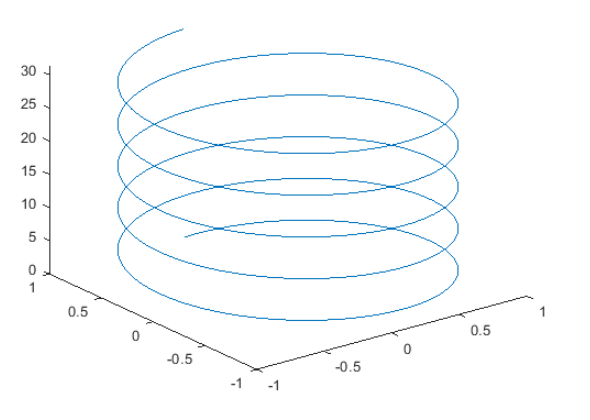
\includegraphics[width=0.7\linewidth]{2}
			\label{fig:2}
		\end{figure}
		
	\end{frame}
\begin{frame}{}
\begin{figure}
	\centering
	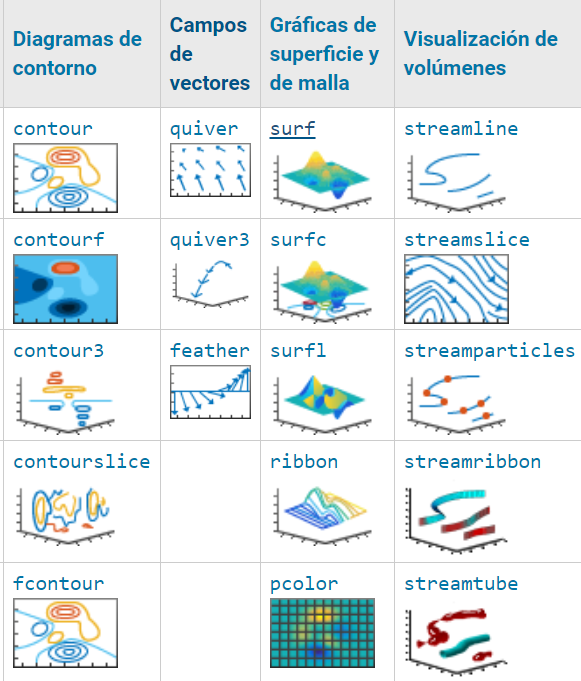
\includegraphics[height=1\textheight]{4}
	\label{fig:4}
\end{figure}
\end{frame}
	\section{Meshgrid}
	\begin{frame}{¿Para qué sirve Meshgrid?}
		\begin{block}{Utilidad}
			la función meshgrid es de suma importancia a la hora de trabajar con datos espaciales generalmente, ya que lo que genera es una grilla, un espacio, lo que finalmente son todas las combinaciones que se pueden hacer entre 2 vectores.
		\end{block}
	\begin{exampleblock}{Dificultades si no se ocupa meshgrid}
		Meshgrid te genera grillas, por lo que si quieres, por ejemplo, trabajar de manera matricial una función f(x,y), en la mayoría de los casos Matlab no podrá trabajar con el espacio XY ya que no está definido, solo tienes vectores x e y
	\end{exampleblock}
	\end{frame}
\begin{frame}[fragile]{Ejemplo}
	\begin{verbatim}
	x=1:100;
	y=1:100;
	[X,Y]=meshgrid(x,y);
	z=X.*Y;
	contour(X,Y,z)
	\end{verbatim}
\begin{figure}
	\centering
	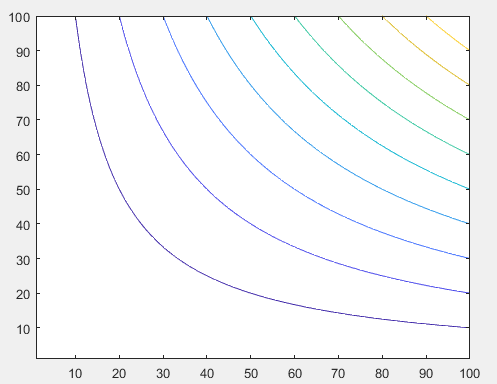
\includegraphics[width=0.5\linewidth]{5}

	\label{fig:5}
\end{figure}

\end{frame}
\end{document}

